\newpage
\subsection*{Question 1}

\begin{enumerate}[label={\alph*)}]
    \item First let's take a look at the 10 lowest latencies for each website:
    
    \begin{center}
        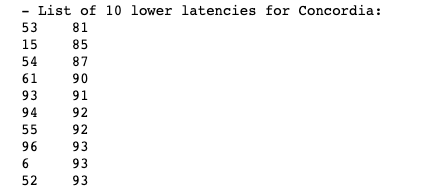
\includegraphics[width=0.5\textwidth]{img/img1.png}
    \end{center}
    \begin{center}
        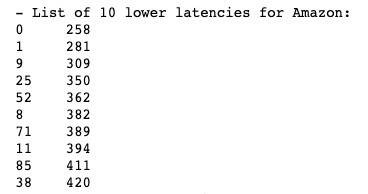
\includegraphics[width=0.5\textwidth]{img/img2.png}
    \end{center}
    
    \noindent Values for Amazon are way higher than those for Concordia. This is confirmed when we take a look at the average latency for each. While requests to \verb|concordia.ca| have an average latency of 110.71ms, those to \verb|amazon.ca| have an average latency of 651.37ms.\\ Since we know there is significantly more successful requests to \verb|concordia.ca|, we want to know if it has an impact on the fact that requests to \verb|amazon.ca| have such a higher latency in average. We find out that successful requests to \verb|amazon.ca| have an average latency of 677.48ms.
    
    \item 100 requests are sent for both websites.
    
    \item Requests to \verb|concordia.ca| were all successfully processed. However, for \verb|amazon.ca| only 62 of the 100 requests were successfully processed. 
    
    \item There are significant differences between results of requests sent to \verb|concordia.ca| compared to those sent to \verb|amazon.ca| both in latency and in success rate. This can be due to the fact that \verb|amazon.ca| protects itself from attacks and hence tend to block requests issued by simulated users. If not, it would be possible to conduct attacks against websites and make them eventually crash if more requests than servers can handle are made. 
\end{enumerate}
